\chapter{线性表}

欢迎来到第二章。


假设某游戏的玩法是玩家操控一个四人组成的小队，队伍成员存在严格有序的位置关系，类似这样：
\begin{bulk}
\begin{center}
邪念 → 银心 → 甘尔 → 张三
\end{center}
\end{bulk}
这，其实就是一个由四个“游戏中的可操控角色”构成的\uwave{线性表}，表中有四个元素，元素的类型是“角色”，可能类似这样：
\begin{cppcodeNum}[label={code:Role类型定义}]
struct Role{
    int hp;             // 生命值
    int attack_power;   // 攻击力
    // ...              // 其他
};
\end{cppcodeNum}
有了这个例子，我们给出如下线性表的定义：
\begin{definitionbox}
    \term{线性表}是具有\uline{相同数据类型}的\(n(n>=0)\)个元素构成的有限\uline{有序}序列，其中\(n\)为表长，当\(n=0\)时线性表是一个空表。
\end{definitionbox}
请注意，线性表所称元素“有序”，这并不是说元素的值大小有序，而是元素有严格的位置关系。例如，我们可以用\(L\)将线性表表示为：
\[
L = (a_1, a_2, ..., a_n)
\]
其中，\(a_1\)是唯一的第一个元素，\(a_n\)是唯一的最后一个元素。

\section{顺序表和链表简介}
线性表最常见的实现方式有两种。在C语言中，我们可以利用数组让这些元素在内存中连续地存放。这种利用一段连续的存储空间依次保存表中元素的线性表被称为\term{顺序表}。
顺序表的存储结构定义如代码\ref{code:线性表的顺序存储结构}所示。
\begin{cppcodeNum}[label={code:线性表的顺序存储结构}, codetitle={线性表的顺序存储结构}]
    #define MaxSize 100
    struct SeqList{  // SeqList, 即Sequential List
        ElemType data[MaxSize];  // 存放表中元素，可用数组下标为0-99
        int current_size;       // 当前表中的元素数量
    };
\end{cppcodeNum}
其对应的物理存储结构如图\ref{fig:顺序存储的线性表}所示。
\begin{figure}[htbp]
    \centering
    % trim: 左 下 右 上
    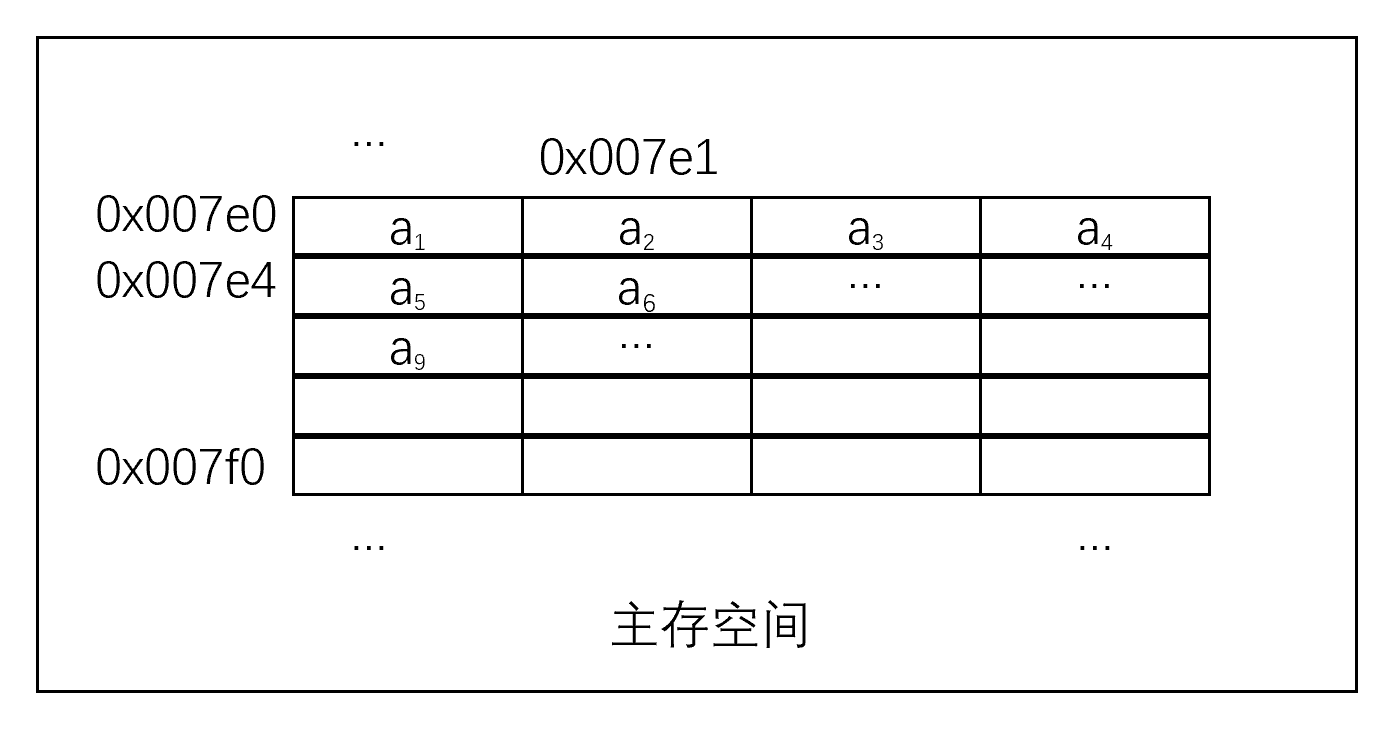
\includegraphics[width=0.55\textwidth, trim=0 1.5cm 0 0]{assets/pics_and_ppts/ch2/顺序存储的线性表.png}
    \caption{顺序存储的线性表}
    \label{fig:顺序存储的线性表}
\end{figure}

\begin{notebox}{初见提示}
相信你懂我的意思，但初见我还是要多啰嗦一句：图\ref{fig:顺序存储的线性表}中我们假设了某顺序表起始地址为0x007e0，每个元素大小为1字节。
而在后续诸多内容中我们将省去这种用于严谨的话术，而专注于“传意”的意图。
\end{notebox}

\begin{notebox}{提示}
代码\ref{code:线性表的顺序存储结构}中，我们用ElemType(Element Type)表示表中的元素类型。比如你要处理一组int型数据，把它们放在线性表中，ElemType就可以是int类型；再比如你要处理四个游戏角色，
ElemType就可以是Role类型(类似代码\ref{code:Role类型定义})。
\end{notebox}
顺序表保证了逻辑上相邻的两个元素物理上也一定相邻。因此，表中任何一个元素的地址都可以由
\begin{bulk}
    \begin{center}
        Address(\(a_i\)) = Address(\(a_1\)) + sizeof(ElemType) \(\cdot\) (\(i-1\)) 
    \end{center}
\end{bulk} 
计算得来。因此，访问（读或写）顺序表中的任意一个元素，都可以在O(1)时间内实现，这种特性我们称为\term{顺序表支持随机访问}。
\begin{insightbox}
若线性表可以对任意元素\(a_i\)进行读写，而且操作时间为\(O(1)\)，与\(i\)和数组大小\(n\)无关，则这种访问方式称
为\term{随机访问（random access）}。如何理解“随机”？第一，可以理解为表可以对任一位序实现O(1)的访问效率，即使位序是“随机”给出的。
第二，与链表做对比。我们将马上看到，链表只能顺序访问（sequential access），而无法随机访问。也就是说，要访问链表中位序为i的元素，
我们必须依次访问\(a_1\), \(a_2\), ..., \(a_{i-1}\), \(a_i\)。而无法跳过前面直接访问\(a_i\)。
\end{insightbox}
不难想到，可以使用如下代码初始化一个顺序表并为其构造元素：
\begin{cppcode}
    // 假设我们要将存放在数组a中，长度为n的数据插入某个顺序表中 
    struct SeqList L;        // 定义一个顺序表
    L.current_size = 0;     // 空表初始元素数量为0
    // 插入数据
    for(int i=0; i<n; i++) {
        if(L.current_size < MaxSize) {    
            L.data[L.current_size] = a[i];  
            L.current_size++;
        } else {
            // 表已满，拒绝插入
        }
    }
\end{cppcode}

通过C语言提供的指针，我们也可以让每个元素通过一个指针指向下一个元素，从而链接起整个线性表。这种通过指针，将一个个物理上未必连续的存储空间链接起来的
线性表被称为\term{链表}。在这种实现方式下，表的每个节点除了存储数据元素本身，还要额外存储一个“指向下一个元素的指针”。因此，我们需要一个struct来
描述表的一个“节点”：
\begin{cppcode}
    struct ListNode{
        ElemType data;  // 该节点的数据元素
        struct ListNode* next_node; // 下一个节点的地址 
    };
\end{cppcode}
\begin{figure}[htbp]
    \centering
    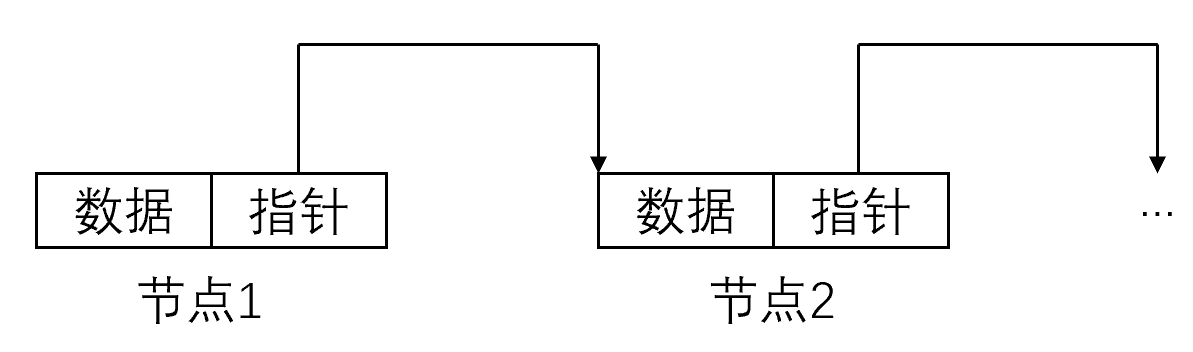
\includegraphics[width=0.5\textwidth, trim=0 1cm 0 0]{assets/pics_and_ppts/ch2/链表的节点.png}
    \caption{链表的节点}
    \label{fig:链表的节点}
\end{figure}
由于有了第一个链表节点的指针，就可以顺着链条找到所有节点，因此，一个链表可以用其第一个节点的指针来表示：我们定义
\begin{cppcode}
    typedef struct ListNode* LinkList;  // LinkList 是指向ListNode的指针类型 
\end{cppcode}
于是，就可以用
\begin{cppcode}
    LinkList L;
\end{cppcode}
来定义一个“链表”对象L（就像用"int a;"来定义一个int型对象a一样）。
\begin{notebox}{提示}
    LinkList与ListNode*是同一种类型。只不过语义上强调的重点不同：ListNode*强调“这是一个节点”，而LinkList强调“这是一个链表”。我们也经常使用
    \begin{bulk}
        typedef struct ListNode* head;
    \end{bulk}
    来突出head是链表第一个节点的指针。
\end{notebox}
链表的物理存储结构如图\ref{fig:链式存储的线性表}所示。
\begin{figure}[htbp]
    \centering
    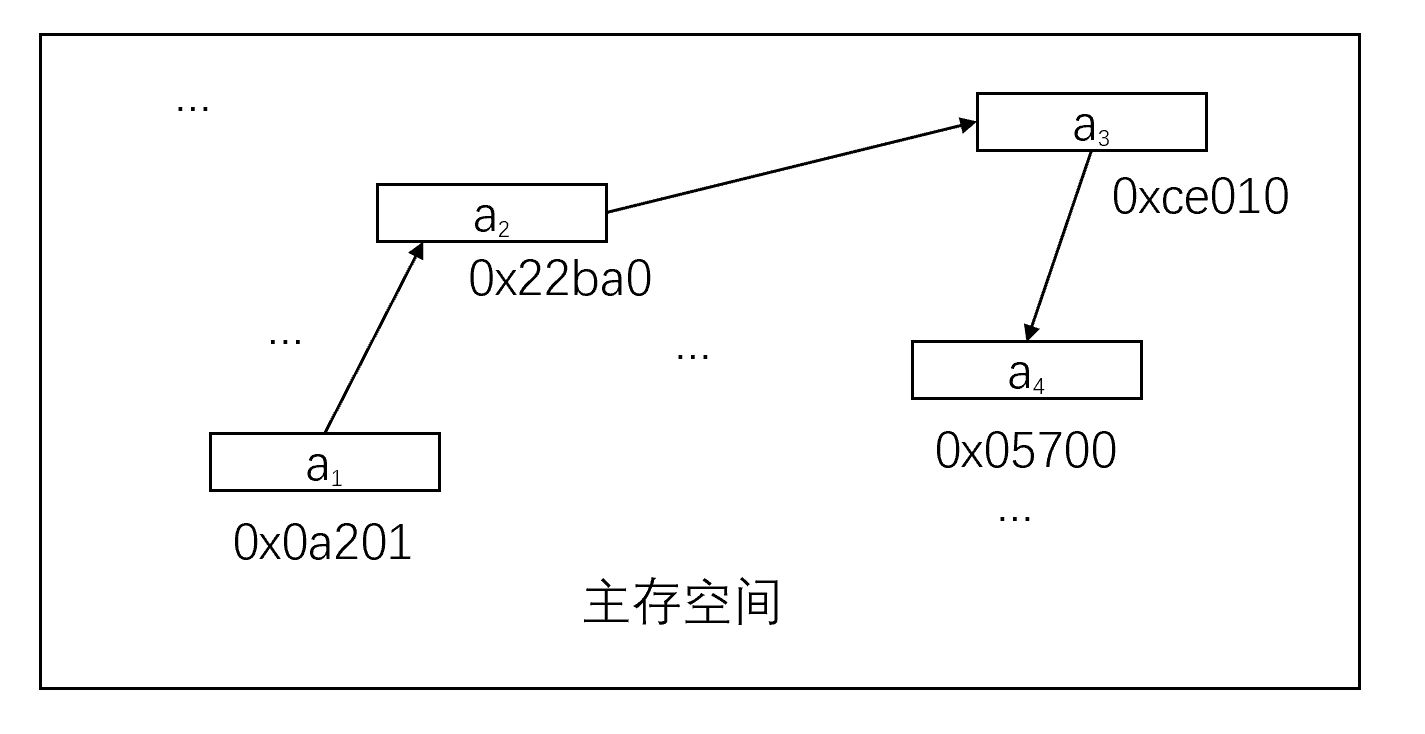
\includegraphics[width=0.55\textwidth, trim=0 1.2cm 0 0]{assets/pics_and_ppts/ch2/链式存储的线性表.png}
    \caption{链式存储的线性表}
    \label{fig:链式存储的线性表}
\end{figure}
现在假设我们要将存放在数组a中，长度为n的数据插入某个链表中，请你尝试写出C语言代码。后面我们会给出更一般化的代码。

\section{顺序表}
经过上面的介绍我们可以看出，顺序表的优点在于：\Circled{1}支持随机访问，访问表中任意元素可以O(1)时间实现；\Circled{2}几乎无需额外存储空间存储额外信息，
不像链表那样需要额外存储n个指针。顺序表的缺点也很明显：插入或删除表中元素时需要移动大量元素。

接下来我们给出顺序表常见操作的代码实现，通过代码大家也可以进一步体会这一点。对于一个未初始化的顺序表L：
\begin{cppcode}
    struct SeqList L;
\end{cppcode}
\minisection{1.顺序表的初始化操作}
顺序表中通过一个整数变量current\_size来维护当前表长（表中已有元素数量）。初始化时，将其置为0：
\begin{cppcode}
    void InitList(struct SeqList *L) {
        L->current_size = 0;
    }
\end{cppcode}
\minisection{2.顺序表的插入操作}
以下函数实现了操作：在顺序表L中，第index个位置插入一个值为value的元素。index=1表示在表头插入。
\begin{cppcode}
    int InsertSeqList(struct SeqList *L, int index, ElemType value) {
    if (L->current_size >= MaxSize) {
        return 0; // 表已满
    }
    if (index < 1 || index > L->current_size+1) {
        return -1; // 插入位置非法
    }
    // 移动元素，为待插元素“腾出位置”
    for (int i = L->current_size; i >= index; i--) {
        L->data[i] = L->data[i - 1];
    }
    // 在第index个位置插入新元素，即数组下标为index-1的位置
    L->data[index-1] = value;
    L->current_size++;
    return 1;
}
\end{cppcode}
插入过程如图\ref{fig:顺序表的插入操作}所示。
\begin{figure}[htbp]
    \centering
    % fbox: 带边框
    \fbox{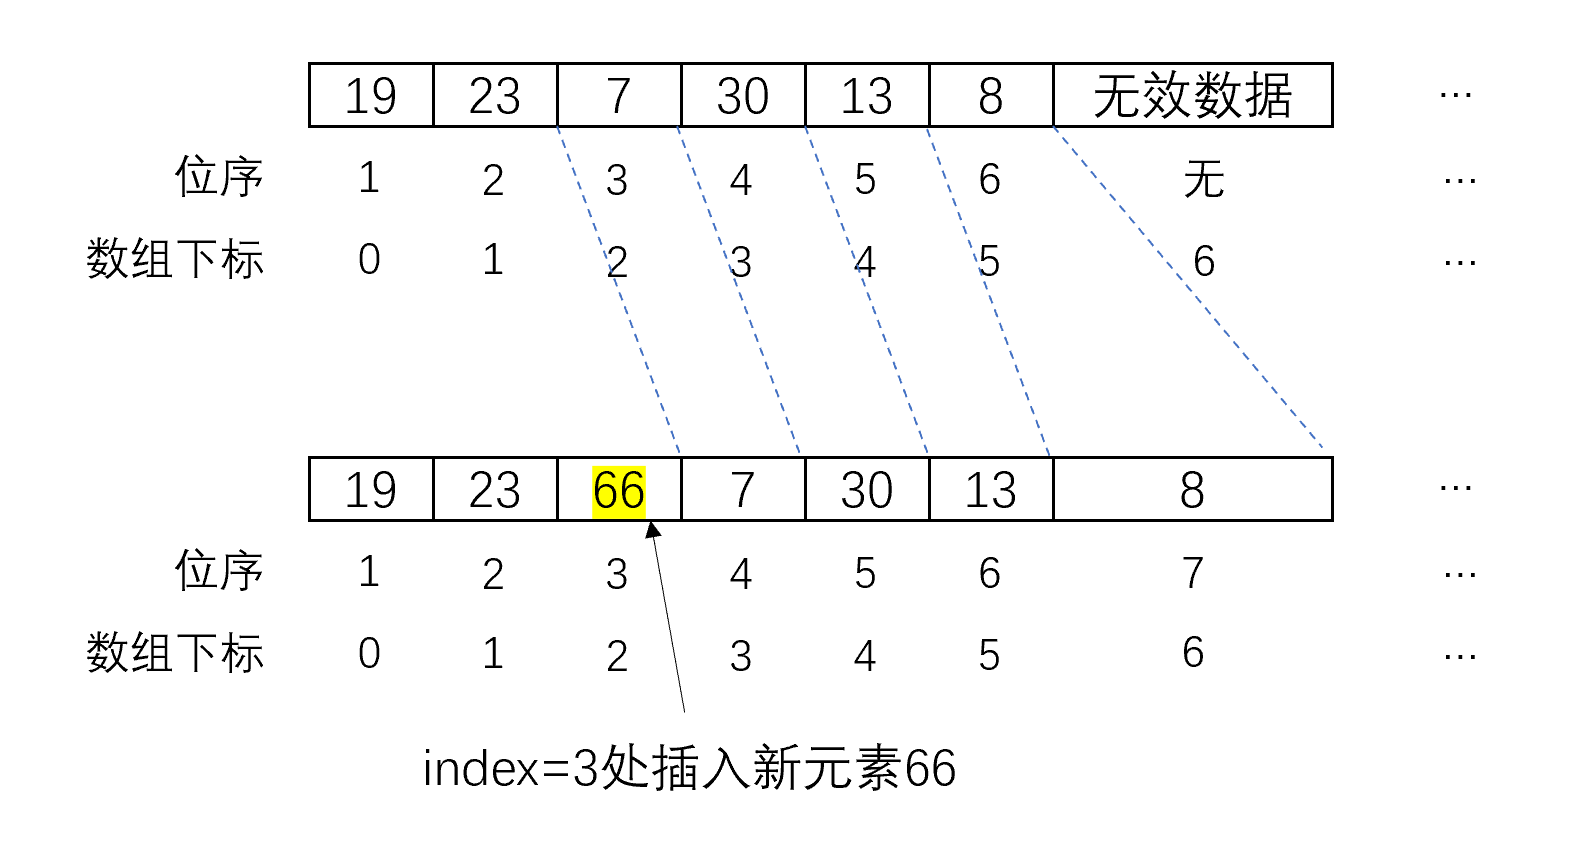
\includegraphics[width=0.55\textwidth]{assets/pics_and_ppts/ch2/顺序表的插入操作.png}}
    \caption{顺序表的插入操作}
    \label{fig:顺序表的插入操作}
\end{figure}
对于顺序表，要在index位置处插入新元素，就要将大量元素依次向右推移一个位置，为新元素腾出位置。显然该算法的瓶颈在于元素移动。不难得出该算法
最好情况下（在表尾插入，无需移动元素）时间复杂度为\(O(1)\)。最坏情况下（在表头插入）元素需要移动n次，\(T(n)=n\)，时间复杂度为\(O(n)\)。
平均情况下，假设在各个位置插入概率相等，则有
\[
    T(n) = \frac{1}{n+1}\cdot 1 + \frac{1}{n+1}\cdot 2 + ... + \frac{1}{n+1}\cdot n = \frac{n}{2}
\]
所以平均情况下，算法时间复杂度为\(O(n)\)。

\minisection{3.顺序表的删除操作}
以下函数实现了操作：将顺序表L中第index个元素删除，并将其值以value变量返回。index=1表示删除表头元素。
\begin{cppcode}
    int DeleteSeqList(struct SeqList *L, int index, ElemType *value) {
    if (index < 1 || index > L->current_size) {
        return -1; // 删除位置非法
    }
    // 将被删元素赋值给变量value
    if (value != NULL) {
        *value = L->data[index-1];
    }
    // 用第index+1个元素（如果有）覆盖第index个元素，并将后面所有元素“前移一格”
    for (int i = index-1; i < L->current_size - 1; i++) {
        L->data[i] = L->data[i + 1];
    }
    L->current_size--;
    return 1;
}
\end{cppcode}
与插入操作的思想类似，显然删除操作的时间复杂度同样为O(n)。
\begin{notebox}{初见提示}
    事实上绝大多数时候我们关注的都是平均复杂度，因此，在未指出“最好”“最坏”或“平均”时，我们提到的“时间复杂度”或“空间复杂度”都是指平均。
\end{notebox}
\begin{insightbox}
    相信这里已经是一个非常合适的位置来指出这几件事：
    \\
    
1.顺序表插入操作的实现代码中，我们规定表满时返回0，插入位置非法时返回-1，插入成功时返回0。为什么要这么规定？为何元素的位序index从1开始算，而不是从0？为何插入操作
名字叫做InsertSeqList？叫别的名字可以吗？
    
    回答：事实上，这些并非死规定，而是由该函数的\uline{实现者}来定义的。如果你来实现这个函数，你当然可以做出其他合理规定，如：“只要插入失败都返回0，只要插入成功就返回1”，
    再如你将函数名起为“SeqListInsert”，这都是可以的，只要你正确地实现了该函数，并给出清晰的说明让该函数的\uline{使用者}知道这个函数具体怎么用就行。类似的事情后面将不再赘述。
    \\
    
2.对于顺序表的删除操作，你也许会问，“删除操作”不就是删掉元素吗？为何还要将被删元素的值返回？这是因为在实际需求中，我们删除一个元素往往需要同时拿到它的值。
    比如，若银心出队去营地休息，我们将她从玩家队伍中移出，可能同时需要将她放入营地，这就需要获取“银心”这一数据元素，因此删除的同时要返回该数据。你当然可以将
    删除操作实现为“只删除，不返回被删元素”，只要你实现得正确。但正如1.1节末尾所指出，本书中每一种数据结构，我们给出的都是较常见的、一般的实现方式。这一点后面将不再赘述。
    \\

    说到这里是时候指出《数据结构》的一个重要思想，请看下面的“3”。
    \\

3.你在解决实际问题时（很可能是某个OJ网站上的问题），在你玩转某个数组的时候，你顺着自己的思路写出的很可能其实就是顺序表的插入、删除等操作，而你决不会把它封装
    成一个函数类似InsertSeqList(...)。但是，《数据结构》的研究在于抽象和封装。
    实际的工程中，你也可以将某个结构及其对应的操作封装好，并和别人说：“这个结构是一棵平衡二叉树，它支持操作123456等、作用分别是xxxxxx，你可以直接拿去用
    （而无需关注其底层是怎么实现的，因为我已经帮你实现好了）”。当然，你最好给出每个接口实现（函数实现）的详细说明，如时间、空间复杂度，各个返回值表示的含义等等。
    相信随着对《数据结构》的研究，你将逐步加深对该思想的体会。
    
\end{insightbox}

\minisection{4.按位序访问/修改元素}
如前所述，顺序表的存储特性决定了它支持随机访问，我们可以直接根据数组下标来访问元素。
\begin{cppcode}
    // 获取位序为index的元素
    int GetElem(struct SeqList *L, int index, ElemType *value) {
        if (index < 1 || index > L->current_size) {
            return -1; // 访问失败
        }
        *value = L->data[index-1];
        return 1;     // 访问成功
    }
    // 将位序为index的元素修改为new_value, 旧值通过value返回
    int SetElem(struct SeqList *L, int index, ElemType new_value, ElemType *value) {
        // 此处略去合法性检查

        *value = L->data[index-1];
        L->data[index-1] = new_value;
        return 1;     // 访问成功
    }
\end{cppcode}
显然该操作时间复杂度为O(1)。
\minisection{5.按值查找元素}
以下函数实现了操作：返回表L中第一个值等于value的元素所在位序。若不存在，返回-1.
\begin{cppcode}
    int SeqListFind(struct SeqList *L, ElemType value) {
        for (int i = 0; i < L->current_size; i++) {
            if (L->data[i] == value) {
                return i+1;
            }
        }
        return -1;
    }
\end{cppcode}
显然该操作时间复杂度为O(n)。{\color{red}\textbf{在后面我们将会看到}}，若顺序表中元素按从小到大或从大到小有序，我们还可以使用\uwave{二分查找}提高查找效率。

到这里我们给出了顺序表的五种常见操作。当然你还可以为它定义更多的操作，如“获取表长”、“判断表是否为空”等操作，感兴趣的同学可以自己尝试实现。
\subsection{从使用者视角理解“数据结构”}
以上我们以“实现者”的视角提供了顺序表这一数据结构及其操作的实现。有了以上实现，我们就有了一个具有基本功能的顺序表可以使用。接下来我们进入“使用者”的视角，
来看一看我们可能会如何使用一个顺序表。我们依然以游戏设计为例。假设你设计的游戏玩法是玩家操控一个四人小队，“出征队伍”最多四人，而你可以随时让“出征队伍”
中的队友去营地休息，也可以随时让营地中的队友加入“出征队伍”。

在你编写代码时，程序启动之初你可能会创建一个用来保存“出征队伍”的顺序表，以及一个用来保存“营地队员”的顺序表并初始化：
\begin{cppcode}
    #define MaxSize 4
    struct RoleSeqList {
        struct Role roles[MaxSize];
        int current_size;
    }
    RoleSeqList expedition_team; // 出征队伍列表
    RoleSeqList camp;    // 营地中的队员列表
    InitList(expedition_team);
    InitList(camp);
\end{cppcode}
游戏之初出征队伍可能只有主角“邪念”一个人，最初你将邪念加入表中：
\begin{cppcode}
    // 假设玩家通过“捏脸”后的数据，或游戏默认的主角初始数据保存在某Role类型的对象"XieNian"中。
    InsertSeqList(expedition_team, 1, XieNian);
\end{cppcode}
而营地中暂时没有队友。随着游戏进行，由于你的好人缘，可能不断有队友“归顺于你”：
\begin{cppcode}
    int result = InsertSeqList(expedition_team, expedition_team.current_size+1, YinXin);    // YinXin入队
    if(result == 0) {
        // 可以在此提示玩家：你的小队最多只能有四个人
    } else if(result == -1) {
        // 错误处理，据实际情况而定
    }
    result = InsertSeqList(expedition_team, ...);   // 其他人入队
    // ...
\end{cppcode}
当你的出征队伍种有了一定数量的人员之后，假设某时刻玩家可能选择让位序为index的人出队并且去营地休息：
\begin{cppcode}
    int result = DeleteSeqList(expedition_team, index, value);  // 位序为index的人出队
    if(result != 1) {
        // ...
    }
    int result = InsertSeqList(camp, camp.current_size, value); // 把这个人放入营地
    if(...) {
        ...
    }
\end{cppcode}
以上便是我们对“顺序表”这一数据结构可能的使用。事实上，游戏中的“出征队伍”和“营地”只是我们为了实现游戏玩法而定义的两个概念。对于顺序表的实现代码来说，
它们并没有什么特殊之处：出征队伍是一个顺序表，营地也是一个顺序表。顺序表并不知道自己保存的Role是何含义，也不知道这些“Role”为什么需要在两个列表之间移动。
它只负责提供一组通用的操作，例如插入、删除、查找和访问。

这正是数据结构的价值所在：我们是在设计一种种通用的数据组织方式，然后在不同的实际问题中重复使用它。

在这个例子中，我们甚至可以进一步把游戏中的具体概念暂时抛开。无论顺序表中存储的是游戏角色、商品，还是其他任何类型的数据，对于顺序表本身而言，它们都只是一个个数据元素。
只要这些元素满足顺序表的基本要求，我们就可以使用同一套数据结构及其操作来管理它们。
因此，从使用者的角度来看，数据结构实际上是一种可以被反复复用的通用工具。它将“如何组织数据”以及“如何操作这些数据”封装起来，使上层程序可以直接利用这些能力
（如直接调用InsertSeqList(camp, camp.current\_size, value)），而不必重复考虑底层的实现细节。这也体现了计算机这门学科一个很重要的思想：“封装”。

至此，相信你已经对《数据结构》这门学科“到底在研究啥”已经有了一个很深刻的认知。此后，除非必要，我们将不再强调类似内容，而专注于《数据结构》本身的研究上。
\section{链表}
在2.1节中我们已经给出了链表存储结构的定义：
\begin{cppcode}
    struct ListNode{
        ElemType data;  // 该节点的数据元素
        struct ListNode* next_node; // 下一个节点的地址 
    };
    typedef struct ListNode* LinkList;
\end{cppcode}
链表的节点通常是通过malloc或new动态分配的，因此逻辑上相邻的节点物理存储上未必相邻。如前所述，我们有了上述定义，就可以像定义一个int变量一样定义一个链表对象my\_linklist。
我们首先给出链表的初始化操作，对于一个定义了但尚未初始化的链表my\_linklist：
\begin{cppcode}
    LinkList my_linklist;  // 此时my_linklist指向未知数据。再次提醒：这个my_linklist语义上既可以表示“一个链表”，也可以表示“该链表的第一个节点指针”
\end{cppcode}
\minisection{1.链表的初始化操作}
初始化一个空的链表，只需要将指向第一个节点的指针置为NULL即可：
\begin{cppcodeNum}[label={code:不带头节点的链表初始化}, codetitle={不带头节点的链表初始化}]
    int InitLinkList(LinkList* L) {
        *L = NULL;
        return 1;
    }
\end{cppcodeNum}
调用
\begin{cppcode}
    InitLinkList(&my_linklist);
\end{cppcode}
即可对my\_linklist这个链表进行初始化。如图\ref{fig:链表初始化前后示意} a）所示。函数将链表第一个节点的指针my\_linklist置为NULL，表示此时表中没有数据元素。
\begin{figure}[htbp]
    \centering
    \fbox{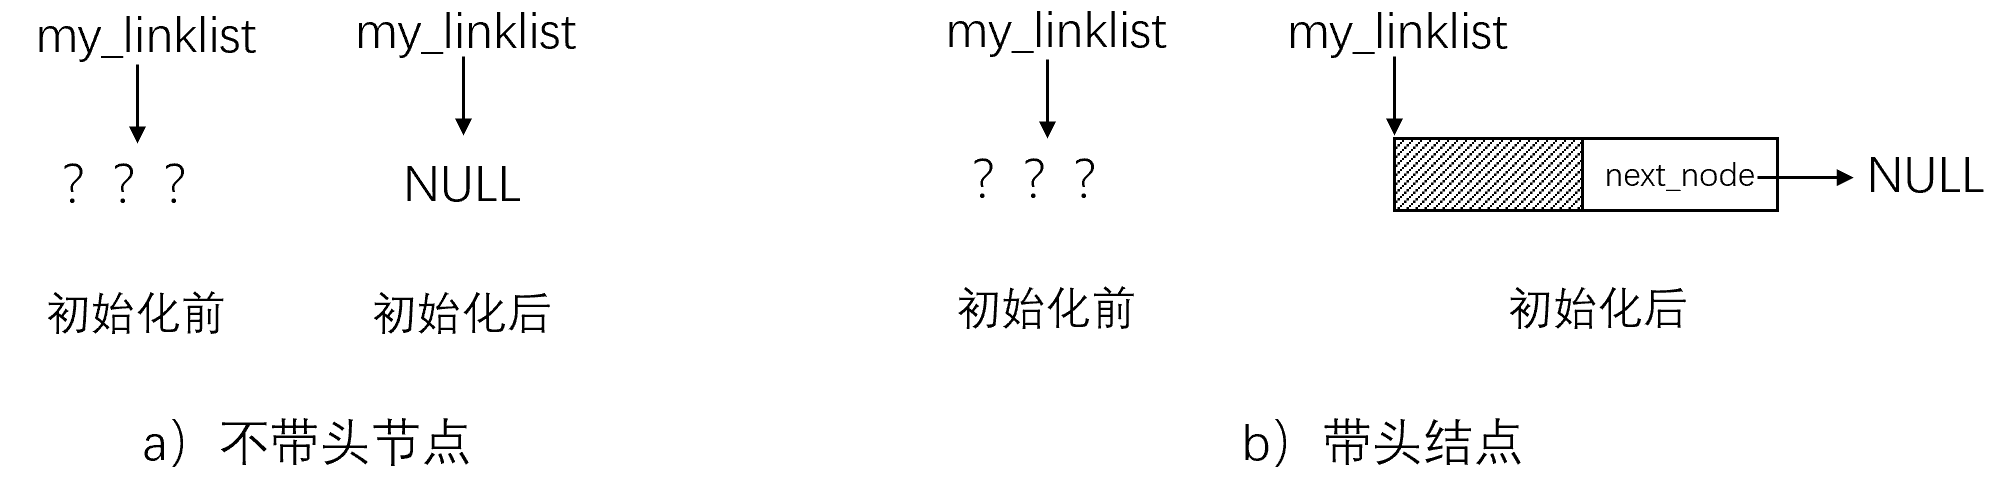
\includegraphics[width=0.78\textwidth]{assets/pics_and_ppts/ch2/链表初始化前后示意.png}}
    \caption{链表初始化前后示意}
    \label{fig:链表初始化前后示意}
\end{figure}
事实上，为了操作上的方便，我们在实现链表时，通常在表的第一个\uline{有效的数据节点}之前附加一个节点，称为\term{头节点}，如图\ref{fig:带头节点与不带头节点的链表}所示。
头节点同样可以用ListNode结构来定义，只不过这个节点不保存有效数据（data字段可以不填值），而仅仅是链表的实现者为了代码简单易实现、不出错而额外引入的一个辅助节点。
\begin{figure}[htbp]
    \centering
    \fbox{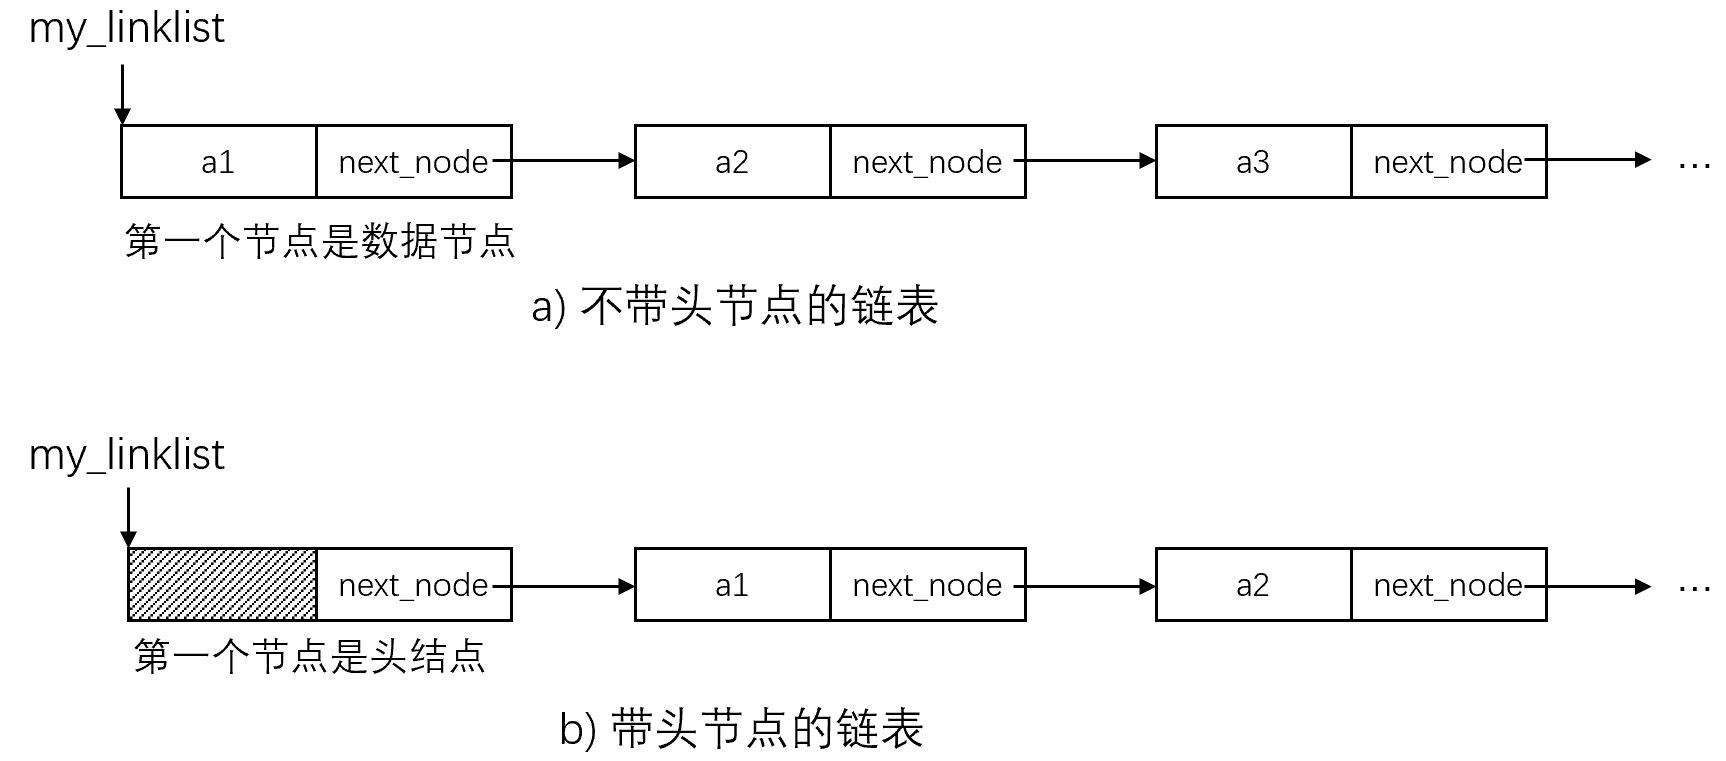
\includegraphics[width=0.9\textwidth]{assets/pics_and_ppts/ch2/带头节点与不带头节点的链表.png}}
    \caption{带头节点与不带头节点的链表}
    \label{fig:带头节点与不带头节点的链表}
\end{figure}

\begin{notebox}{提示}
    （特别是北方的朋友）请注意，对于带\term{头节点}的链表，头节点确实等同于“头一个节点”，即第一个节点。而对于不带\term{头节点}的链表，不能把第一个节点叫做“头节点”，
    “头节点”是一个专有名词，而不是表达“头一个节点”的语义。
\end{notebox}

引入了头节点后，头节点即第一个节点，因此对于带头节点的链表，第一个节点的指针就是指向头节点的指针。带头节点的链表初始化操作代码如下：
\begin{cppcodeNum}[label={code:带头节点的链表初始化}, codetitle={带头节点的链表初始化}]
    int InitLinkList(LinkList* L) {
        *L = (ListNode*)malloc(sizeof(ListNode));    // 创建头节点
        if(*L == NULL) {
            return 0;
        }
        (*L)->next_node = NULL;    
        return 1;
    }
\end{cppcodeNum}
初始化过程如图\ref{fig:链表初始化前后示意} b）所示。

\begin{notebox}{提示}
    在代码\ref{code:不带头节点的链表初始化}及代码\ref{code:带头节点的链表初始化}中，LinkList本身类型是ListNode*，因此LinkList* 的类型是ListNode**,
    是一个二级指针。所以*L类型是ListNode*，即指向某链表节点的指针。
    
    要在函数栈内改变栈外普通变量的值就要用其指针作为参数传递。而栈外的变量my\_linklist本身是一个指针，因此要在函数栈内改变其值，就要用指针的指针。

    如果你熟悉C++，就可以使用C++中的引用传参来解决多级指针带来的理解上的问题。后续内容中在一些地方我们将使用引用降低语言本身带来的理解负担，这样可以将更多精力专注于
    《数据结构》本身的思想。
\end{notebox}
由于带头结点的链表更常用，如无特殊说明，本节中均默认链表带头结点。

\minisection{2.销毁链表}
销毁链表与初始化相对应。销毁链表需要释放每个节点的内存空间。
\begin{cppcode}
    void DestroyLinkList(LinkList* L) {
        struct ListNode* p = *L;    // p始终指向当前待释放位置
        struct ListNode* q;
        while (p != NULL) {
            q = p->next_node;       // q是下一个待释放位置
            free(p);
            p = q;
        }
        *L = NULL;
    }
\end{cppcode}
这里需要注意，第7行不能写成“p = p->next\_node”。因为p在第6行已经被释放了，再访问p会导致未定义行为。这也是为什么要先用q保存p的值。
\minisection{3.判断链表是否为空}
由于我们采用的是带头结点的设计，因此第一个节点的next\_node指针指向的才是实际的第一个数据元素节点。
\begin{cppcode}
    int ListIsEmpty(LinkList L) {
        return L->next_node == NULL;
    }
\end{cppcode}

\minisection{4.求链表长度}
求链表长度的操作是计算链表中数据节点的个数。对于链表，我们想要求得表长就需要遍历一遍链表，每访问到一个有效的数据节点就将计数器加一，最后得到表长。
\begin{cppcode}
    int GetLength(LinkList L) {
        int length = 0;
        struct ListNode* p = L->next_node;  
        while (p != NULL) {
            length++;
            p = p->next_node;
        }
        return length;
    }
\end{cppcode}
显然求链表长度操作的时间复杂度为O(n)。另外请注意，链表长度是不包括头结点的，这一点很好理解。

\begin{insightbox}
    事实上，我们可以对LinkList类型做进一步的封装，类似：
    \begin{cppcode}
        struct WrappedLinkList {
            LinkList L;
            int elem_num;   // 额外增加的变量
        };
    \end{cppcode}
    通过额外维护一个变量elem\_num实时记录当前链表的元素数量，链表初始化时该变量赋值0，插入时加一，删除时减一。这样可以做到O(1)时间求链表的长度。熟悉C++的同学
    可以知道，C++标准库中的std::list就是采用了类似的实现方式，所以std::list的size()方法时间复杂度为O(1)。
\end{insightbox}

\minisection{5.在第i个位置插入元素}
在链表L中的第i个位置插入一个值为e的新节点s，需要断开原来的链条，将新元素“链接上”，其过程如图\ref{fig:链表的插入过程示意}所示。
\begin{figure}[htbp]
    \centering
    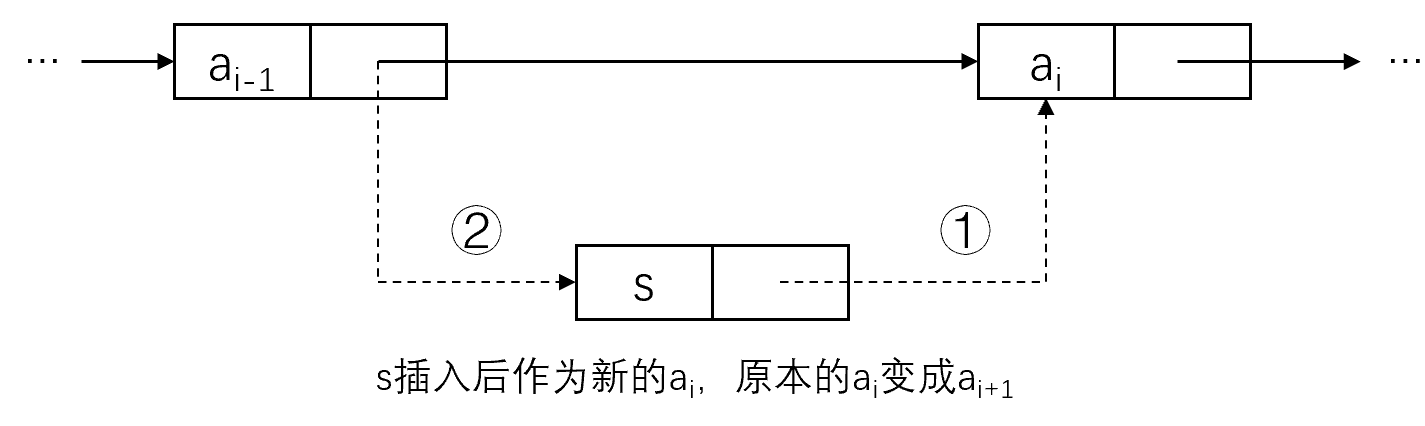
\includegraphics[width=0.7\textwidth]{assets/pics_and_ppts/ch2/链表的插入过程示意.png}
    \caption{链表的插入过程示意}
    \label{fig:链表的插入过程示意}
\end{figure}
实现代码如下。
\begin{cppcode}
    int ListInsert(LinkList L, int i, ElemType e) {
        struct ListNode* p = L;
        // 找到第 i-1 个节点
        for (int j = 1; j < i; j++) {
            if (p->next_node == NULL)
                return 0;   // 插入位置有误
            p = p->next_node;
        } // 该循环结束后，p指向第i-1个节点@\(a_{i-1}\)@
        // 创建新节点
        struct ListNode* s = (struct ListNode*)malloc(sizeof(struct ListNode));
        s->data = e;
        // 插入节点
        s->next_node = p->next_node;    // @\Circled{1}@
        p->next_node = s;               // @\Circled{2}@
        return 1;
    }
\end{cppcode}
可以看到在第i个及第i-1个节点之间插入，要操作链条，就要拿到这两个节点的信息。这也是该算法的主要开销：找到这两个节点的指针。
不难看出该算法时间复杂度为O(n)。通过该例大家也能出头结点所带来的好处之一——简化边界处理：即使插入位置是表首，也不需要特殊处理。
\begin{notebox}{初见提示}
    相信你发现了，代码第十行我们分配内存后没检测是否分配成功。在之后的诸多场景，我们将略去类似代码，而专注于算法的核心思想上。
\end{notebox}

\minisection{6.删除第i个元素}
同插入操作的思想类似，删除操作的核心同样是链条操作，如图\ref{fig:链表的删除过程示意}。
\begin{cppcode}
    int ListDelete(LinkList L, int i, ElemType* e) {
    struct ListNode* p = L;
    struct ListNode* q;
    // 找到第 i-1 个节点
    for (int j = 1; j < i; j++) {
        if (p->next_node == NULL)
            return 0;
        p = p->next_node;
    }
    if (p->next_node == NULL)
        return 0;
    q = p->next_node;
    if (e != NULL)
        *e = q->data;
    // 删除节点
    p->next_node = q->next_node;
    free(q);
    return 1;
}
\end{cppcode}
显然该算法时间复杂度同样为O(n)。
\begin{figure}[htbp]
    \centering
    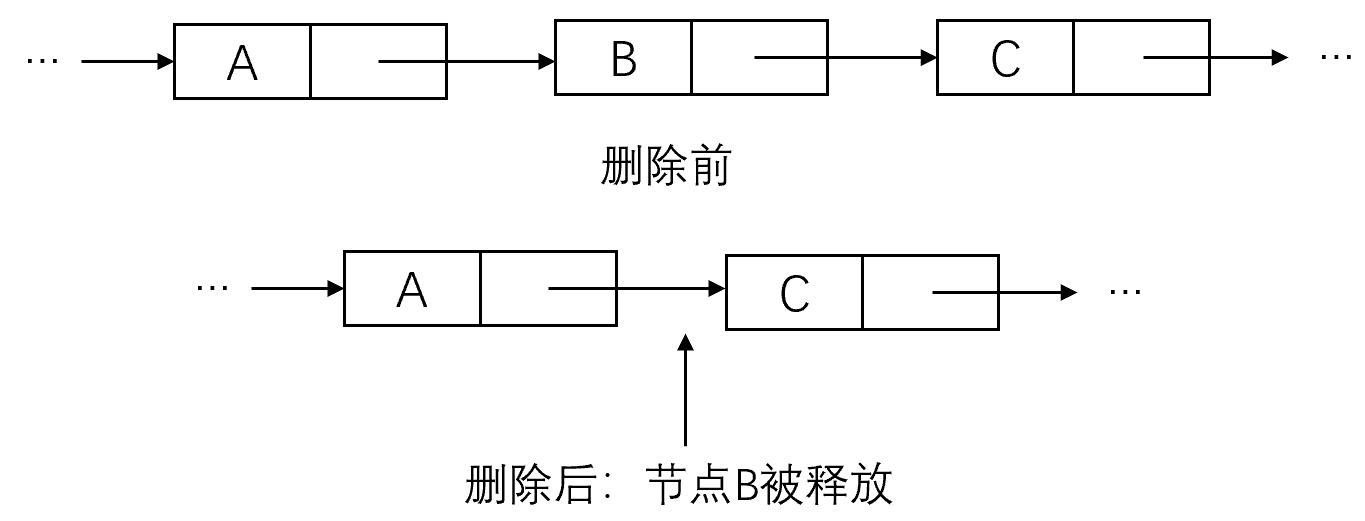
\includegraphics[width=0.7\textwidth]{assets/pics_and_ppts/ch2/链表的删除过程示意.png}
    \caption{链表的删除过程示意}
    \label{fig:链表的删除过程示意}
\end{figure}

\minisection{7.按位置获取元素}
由于链表的存储结构，其无法直接通过访问位置i计算得到元素的地址，而只能从第一个节点顺着链条一个一个往下找。代码实现如下：
\begin{cppcode}
    int GetElem(LinkList L, int i, ElemType* e) {
        struct ListNode* p = L->next_node;
        // 控制指针p始终指向第j个数据节点，j==i成立时，循环结束，p指向第i个节点，即要找的节点
        for (int j = 1; j < i; j++) {
            if (p == NULL)
                return 0;
            p = p->next_node;
        }
        if (p == NULL)
            return 0;
        *e = p->data;
        return 1;
    }
\end{cppcode}
前面我们说链表只能顺序访问（sequential access），而不能随机访问（random access），这里我们也从代码的角度进一步认识了这一点。并且同时我们
不难看出，要修改位序为i的节点，思想和该GetElem函数非常相似，只不过把获取元素变成了修改元素。

至此，我们已经对链表进行了较为深入的探讨。请大家注意，以上我们所谈的“链表”也可以叫做\term{“单链表”}，因为它只有由前指向后的一条“单链”，而没有由后指向前的链条。
事实上，链表还有多种变态，用于灵活地适应不同需求，我们将在{\color{red}\textbf{接下来的章节中展开讨论}}。




\section{顺序表与单链表的对比}
顺序表和单链表都是线性表的常见实现方式，它们都能够表示一组具有线性关系的数据。二者最大的区别在于数据的存储方式不同：
\begin{itemize}
    \item 顺序表使用一段连续的存储空间保存数据，元素之间通过下标表示逻辑关系；
    \item 链表通过指针将多个离散存储的结点连接起来，元素之间通过指针表示逻辑关系。
\end{itemize}
这种存储方式的不同，决定了二者具有不同的特点。
\subsection{随机访问}
由于顺序表中的元素连续存储，因此可以通过下标直接计算元素地址，访问任意位置的元素只需要 $O(1)$ 时间。
因此，顺序表适合需要频繁随机访问的场景。

而单链表中的结点在内存中通常不是连续存储的，无法根据位置直接计算地址。如果想访问第 $i$ 个元素，必须从第一个结点开始依次遍历，因此时间复杂度为 $O(n)$。
\subsection{插入和删除}
\label{subsec:插入和删除}
顺序表在插入或删除元素时，通常需要移动若干元素。因此，顺序表的插入和删除操作平均时间复杂度为 $O(n)$ 。


而链表中的结点通过指针连接。
插入元素只需要修改相关结点的指针关系，就可以完成插入或删除操作，不需要移动其他元素。在已经拿到节点指针的情况下，单链表的插入操作时间复杂度为 $O(1)$，但删除操作
的时间复杂度仍然为O(n)。
即使没提供节点指针，而只提供了插入位序i：ListInsert(LinkList L, int i, ElemType e); 此时虽然插入的时间复杂度为O(n)，但是该算法的主要开销在于找到插入位置，主要
操作是“比较”，而非“移动”，因此虽然都是O(n)，但链表的插入或删除操作也比线性表更快。


\subsection{空间利用}
顺序表需要一段连续的存储空间，并且通常需要提前申请一定容量。如果申请空间过大，会造成浪费；如果空间不足，则可能导致一些后果。

而链表不要求连续存储空间，可以根据需要动态创建结点，因此空间利用更加灵活。但是，链表中的每个结点需要额外保存指针信息，因此会增加额外的存储开销。


\subsection{如何选择}
顺序表和链表没有绝对的优劣，它们分别适用于不同的问题场景。二者总结如下表：

\begin{center}
\begin{tabular}{c|c|c}
 & 顺序表 & 链表 \\
\hline
存储方式 & 连续存储 & 离散存储 \\
随机访问 & $O(1)$ & $O(n)$ \\
插入删除 & $O(n)$ & $O(1)$或$O(n)$，但更快\\
空间利用 & 不灵活 & 动态申请,较灵活 \\
额外空间开销 & 较小 & 需要保存指针,较大 \\
\end{tabular}
\end{center}

因此：

\begin{quote}
如果程序需要频繁访问任意位置的数据，顺序表通常更加合适；

如果程序需要频繁进行插入和删除操作，链表通常更加合适。

...
\end{quote}

通过本节内容也给了我们一个启示：数据结构的设计，甚至很多工程上的设计，都是在不同需求之间进行权衡，一种设计提高了某方面的表现，通常也会付出其他方面的代价。
我们要在不同需求场景下灵活地进行取舍。

\begin{insightbox}
    请你思考这样一个问题：遍历线性表，如以下伪代码：
    \begin{cppcode}
        void TravelList(List L) {
            for( every data in L ) {
                do_something();
            }
        }
    \end{cppcode}
    顺序表和链表哪个更快？\\
    
    我们先来看二者的遍历代码。顺序表的遍历：
    \begin{cppcode}
        for (int i = 0; i < n; i++) {
            visit(arr[i]);
        }
    \end{cppcode}
    每次访问arr[i]前，要计算其地址：arr[i]=arr[0]+(i-1)*sizeof(ElemType). 之后访问内存；链表的遍历：
    \begin{cppcode}
        Node* p = head;
        while (p != NULL) {
            visit(p->data);
            p = p->next;
        }
    \end{cppcode}
    可以看到，链表的遍历是没有乘法操作的。从硬件角度讲，乘法操作是一种很慢的操作。那是不是链表的遍历就比顺序表快呢？并不是。

    我们还要考虑一点：现代计算机有一个非常重要的机制：\term{Cache（高速缓存）}。大家如果了解过《计算机组成原理》或《操作系统》相关内容应该已经恍然大悟了。

    什么是Cache（高速缓存）？这其实也是这门学科一个非常重要的思想，操作系统的实现、高并发服务的架构设计等许多场景下都有Cache的思想。它基于一个经验性
    规律，叫做\term{程序的局部性原理}：

    程序在运行过程中，访问的数据和指令往往不是随机分布的，而是在一段时间内集中访问某些局部区域。具体来说：
    \begin{itemize}
        \item 如果一个数据或指令最近被访问过，那么它近期很可能再次被访问。
        \item 如果一个数据被访问，那么它附近的数据近期也很可能被访问。
    \end{itemize}
    Cache的设计思想就是，将部分“近期可能频繁被访问的数据”装入更高速的设备中，来提升程序的运行性能。举个例子，某大型3D游戏的地图非常大，有10个GB，
    程序并非会将所有地图数据都装入主存，而是只装载玩家所在位置附近的地图，玩家移动到新区域或进行传送等操作，再进行主存和磁
    盘的“数据交换”，将新区域的地图装入主存。在这个场景下，我们可以称“主存”是“磁盘”的“Cache（高速缓存）”。\\

    事实上，现代计算机都会有比内存更高速的缓存，通常称作CPU Cache。根据局部性原理，将近期常用的指令和数据从主存装入CPU Cache，来提升程序的运行性能。
    说到这里，大家应该发现了，对于顺序表，由于其物理连续的存储特性，它的“局部性”是更好的。同一个顺序表极有可能同时被装入CPU Cache。而链表则不同，遍历链表
    时，会发生频繁的CPU Cache和主存的“数据交换”，这种“抖动”会带来极大的性能损耗。\\

        顺序表虽然存在乘法操作，但其局部性更好，而且，现代编译器通常会做出非常棒的编译优化，对于顺序表的遍历代码，可以将乘法操作带来的影响降得很低很低。所以，
    对于遍历操作，顺序表和链表哪个更好，这个问题没有统一的结论，但通常我们认为，在数据量较大时，顺序表的遍历是更快的。
\end{insightbox}


\clearpage%%%%%%%%%%%%%%%%%%%%%%%%%%%%%%%%%%%%%%%%%%%%%%%%%%%%%%%%%%%%%%%%%%%%%%%%%%%%%%%%%%%%%%%%%%%%%%%%%%%%%%%%%%%%%%%%%%%%%%%%%%%%%%
\begin{exercise}
1. 关于线性表，下列说法正确的是（　）。\\
A. (银心, 甘尔, 张三) 和 (甘尔, 银心, 张三)是两个相同的线性表 \\
B. 线性表是一种物理结构，线性表的所有元素物理地址一定连续\\
C. 同一个线性表中各个元素的数据类型可以不同\\
D. 不同线性表的数据元素类型可以不同\\

2. 对于顺序表，假设表中已有 \(n\) 个元素，下列操作中时间复杂度一定为 \(O(1)\) 的是（　）。\\
A. 在表中某位置插入一个元素\\
B. 删除表头元素\\
C. 获取第 \(i\) 个位置上的元素\\
D. 查找值为 \(x\) 的元素\\

3. 对于一个带头结点的单链表：
\begin{bulk}
head → A → B → C → NULL
\end{bulk}
若 p 指向节点 A，现在希望在 A 后面插入节点 X，正确的核心操作是（　）。\\
A. p->next\_node = X;
X->next\_node = p->next\_node;\\
B. X->next\_node = p;
p->next\_node = X;\\
C. X->next\_node = p->next\_node;
p->next\_node = X;\\
D. p = X;
X->next\_node = p->next\_node;\\

4. 以下单链表的操作中，时间复杂度一定是O(1)的是（  ）。\\
A. 求表长\\
B. 在表头插入元素\\
C. 在表尾插入元素\\
D. 获取第\(i\)个位置上的元素\\

5. 在\coderef{code:线性表的顺序存储结构}中，我们存储顺序表元素使用的数组是静态存储的，定义其最大存储数量为100.若存满了，则无法再扩充。事实上，
我们可以使用malloc动态分配数据元素的存储空间，而只保存一个该空间的起始地址指针：
\begin{cppcode}
    struct SeqList{  
        ElemType* data;         // 数组起始地址
        int current_size;       // 当前表中的元素数量
        // ...
    };
\end{cppcode}
请你想一想，动态存储下，会有哪些操作和静态存储不同？（重点思考一下插入操作）\\

6. 假设数组a中下标0-9处存放了10个int型数据\(a_1\)-\(a_{10}\)，请你用数组a中的数据分别构建以下两个链表，填充对应代码：

1） \(a_1\) → \(a_2\) → ... → \(a_{10}\)
\begin{cppcode}
    LinkList f1(int a[], int n=10) {

    }
\end{cppcode}
2） \(a_{10}\) → \(a_9\) → ... → \(a_1\)
\begin{cppcode}
    LinkList f2(int a[], int n=10) {

    }
\end{cppcode}
建议采用带头结点的实现。\\

7. 请你实现一个算法DeleteValue(LinkList L, ElemType e)，删除带头结点的单链表L中所有值等于e的节点。\\




% 8. 【某年408真题】已知一个带头节点的单链表，节点结构为
% \begin{cppcode}
%     struct ListNode {
%         ElemType data;
%         ListNode* link;
%     };
% \end{cppcode}
% 假设该链表只给出了头指针list。在不改变链表的前提下，请设计一个尽可能高效的算法，查找链表中倒数第k个位置上的节点（k为正整数）。若查找成功，算法输出
% 该节点的data域的值，并返回1；否则，只返回0.要求：\\
% 1）描述算法的基本设计思想；\\
% 2）描述算法的详细实现步骤；\\
% 3）根据设计思想和实现步骤，采用C、C++或Java语言实现算法，关键之处给出简要注释。\\

8. 假设线性表采用带头结点的单链表保存，结点定义如下：
\begin{cppcode}
    typedef struct node
    {
        int data;
        struct node *next;
    }NODE;
\end{cppcode}
请你设计一个尽可能高效的算法，对于任意输入的链表L，都能返回其中间节点。
当表长为奇数时，返回中间的那个节点；当表长为偶数时，返回中间两个节点中左边（位序更小）的那个；当表为空表时，返回空指针NULL。\\

9. 

1）请你设计实现将带头结点的单链表逆置的算法。即：将
\begin{bulk}
    \begin{center}
        head → \(a_1\) → \(a_2\) → ... → \(a_n\)
    \end{center}
\end{bulk}
变为
\begin{bulk}
    \begin{center}
        head → \(a_n\) → \(a_{n-1}\) → ... → \(a_1\)
    \end{center}
\end{bulk}

2）设计实现将不带头结点的单链表逆置的算法。\\


10. 【某年408真题】设线性表：
$$ L=(a_1,a_2,a_3,\cdots,a_{n-2},a_{n-1},a_n) $$
采用带头结点的单链表保存，链表中的结点定义如下：
\begin{cppcode}
    typedef struct node
    {
        int data;
        struct node *next;
    }NODE;
\end{cppcode}

请设计一个空间复杂度为 \(O(1)\) 且时间上尽可能高效的算法，重新排列 \(L\) 中的各结点，得到：
$$ L'=(a_1,a_n,a_2,a_{n-1},a_3,a_{n-2},\cdots) $$
要求：\\
1）给出算法的基本设计思想；\\
2）根据设计思想，采用 C 或 C++ 语言描述算法，关键之处给出注释；\\
3）说明所设计算法的时间复杂度。\\
\end{exercise}
\clearpage


% 给出习题答案。exerciseanser部分的内容会被main.tex中的\printanswers收集并打印。
\begin{exerciseanswer} 
1. D。线性表要求元素存在位置上的逻辑关系，A错误；线性表是一种逻辑结构，通常可以用数组或链表实现，B错误；线性表要求同一个表中的数据类型相同，C错误；实际需求中我们
要处理int型的数据，就会使用一个int型的线性表，要处理Role类型的数据，就会使用Role类型的线性表，D正确。\\

2. C。A、B选项都需要移动若干元素，时间复杂度为O(n)；D项需要从表头开始，将每一个元素的值与x对比直至找到，时间复杂度为O(n)。C项，由于每个元素
的地址可以由其位序直接计算得来，因此时间复杂度为O(1)。\\

3. C。\\

4. B。由于链表结构中保存有表首元素指针，因此在表头插入元素时间复杂度一定是O(1)。对于C选项，要在单链表的表尾插入元素，需要先遍历链表，拿到尾节点的指针，再
操作链条，时间复杂度为O(n)。我们将在后面看到，为了解决单链表无法高效在尾部插入元素的问题，可以通过单链表的多种变态解决，如：记录尾指针的
\uwave{循环单链表}、\uwave{循环双链表}等。\\

5. 事实上，这种存储方式下，还需要一个字段capacity标记当前已动态分配的空间总量：
\begin{cppcode}
    struct SeqList {
        ElemType* data;     // 数组起始地址
        int current_size;  // 当前表中的元素数量
        int capacity;      // 当前已分配的数组容量
    };
\end{cppcode}
例如：capacity = 100，current\_size = 80表示分配了100个位置的内存空间，目前使用了80个，还剩20个。操作方面，显然，初始化动态分配版本的顺序表需要
为data分配一个初始空间，初始分配多大你可以自己定义。除初始化外，这里我们仅指出一个重点操作：插入。 

回忆静态存储的顺序表，若表满，只能拒绝插入（当然你可以规定淘汰算法，接受新值淘汰旧值，这取决于你，但静态存储已经无法存储更多了）。而动态存储版本，
当已分配空间满了的时候，我们可以申请一块更大的内存空间，将已有表中数据整体拷贝过去，并接受新元素。C++中的std::vector就采用了类似机制实现。\\

6. 拟采用带头节点的实现。代码如下：

1）要构建\(a_1\) → \(a_2\) → ... → \(a_{10}\)，不难想出，只需要按顺序将每一个元素依次链接到链表尾部就可以，代码如下：
\begin{cppcode}
    LinkList f1(int a[], int n = 10) {
        // 创建头结点
        LinkList head = (int*)malloc(sizeof(ListNode));
        head->next_node = NULL;     
        // 动态维护tail，让其始终指向当前链表最后一个节点
        LinkList tail = head;
        for (int i = 0; i < n; i++) {
            LinkList node = (int*)malloc(sizeof(ListNode));   // 为新数据分配一个节点
            node->data = a[i];
            node->next_node = NULL;
            // 新节点插入在最后一个节点之后（尾插）
            tail->next_node = node;
            tail = node;    // 动态维护tail指针，让tail始终指向最后一个节点
        }
        return head;
    }
\end{cppcode}

    2）要构建\(a_{10}\) → \(a_9\) → ... → \(a_1\)，实际也很简单，只需要按顺序将每一个元素依次插入链表头部即可，代码如下：
    \begin{cppcode}
        LinkList f2(int a[], int n = 10) {
            // 创建头结点
            LinkList head = new ListNode;
            head->next_node = NULL;
            for (int i = 0; i < n; i++) {
                LinkList node = new ListNode;
                node->data = a[i];
                // 新节点插入在头结点之后（头插）
                node->next_node = head->next_node;
                head->next_node = node;
            }
            return head;
        }
    \end{cppcode}
    事实上，函数f1就是许多经典教材中\term{“尾插法”}的实现，函数f2就是\term{“头插法”}的实现。\\


7. 思路：遍历一遍链表，“检查”每一个节点的值，若等于e，将其删除，并重构该节点附近链条。代码如下。
\begin{cppcode}
    void DeleteValue(LinkList L, ElemType e) {
        ListNode* pre = L;          // 当前“检查”的节点的前驱节点
        ListNode* cur = L->next_node; // 当前“检查”的节点
        while (cur != NULL) {
            if (cur->data == e) {
                ListNode* temp = cur;
                // 重构链条
                pre->next_node = cur->next_node;
                // 推移cur指针，准备检查下一个节点
                cur = cur->next_node;
                // 释放删除节点
                free(temp);
            }
            else {
                // 当前节点不是目标节点
                // 前驱和当前节点同时后移, 继续检查下一个节点
                pre = cur;
                cur = cur->next_node;
            }
        }
    }
\end{cppcode}

8. 相信大家很自然地就能想到的一种做法是：先遍历一遍链表，计算出表长n，再从头开始查找\(\frac{n+1}{2}\)位置处的节点将其返回。代码如下：
\begin{cppcode}
    NODE* FindMiddle1(NODE *L) {
        int n = 0;
        // 第一次遍历，统计节点数量
        NODE *p = L->next;  // 带头结点，L->next是第一个数据节点
        while(p != NULL) {
            n++;
            p = p->next;
        }
        // 空表情况
        if(n == 0)
            return NULL;
        // 第二次遍历，寻找第(n+1)/2个节点
        int pos = (n + 1) / 2;
        p = L->next;    // p指针重置为第一个数据节点，从这里开始找
        for(int i = 1; i < pos; i++) {
            p = p->next;
        }
        return p;
    }
\end{cppcode}

事实上，还有一种更高效的算法，就是所谓的经典的\term{“双指针算法”}。我们设置两个指针，slow指针每次走一步，fast指针每次走两步，这样，slow“走过的里程”永远是fast的
一半，所以，当fast走到表尾时，slow就处在中间。需要注意的就是边界判断及奇偶的处理。代码如下：
\begin{cppcode}
    NODE* FindMiddle2(NODE *L) {
        NODE *slow = L->next;
        NODE *fast = L->next;
        if(slow == NULL)
            return NULL;
        while(fast->next != NULL && fast->next->next != NULL) {
            slow = slow->next;
            fast = fast->next->next;
        }
        return slow;  
    }
\end{cppcode}

9. 本题思路很简单。对于带头节点的单链表，我们依次将（本来就在头节点后的\(a_1\)、）\(a_2\)、\(a_3\)、...、\(a_n\)插入到第一个数据节点之前（即头节点之后）就行。
我们动态维护指针p，让其指向当前“待插”节点。代码如下。
\begin{cppcode}
    NODE* Reverse(NODE* L) {
        NODE* p = L->next;  // L是头节点，L->next是第一个数据节点
        L->next = NULL;     // 插入过程中，让链表的“已定形部分”的尾节点指向NULL
        while(p) {
            // next为下一个待插节点
            NODE* next = p->next;
            // 插入当前节点
            p->next = L->next;
            L->next = p;
            // 动态维护p，使其指向下一个待插节点
            p = next;
        }
        return L;
    }
\end{cppcode}
这个过程其实也可以理解为按顺序将当前链表节点用头插法{\color{red}\textbf{（见习题1 第6小题）}}“重新插入该链表”。

对于不带头结点的单链表同样是将每一个节点依次插入到第一个数据节点之前：
\begin{cppcode}
    NODE* Reverse(NODE* L) {
        NODE *new_head = NULL;
        NODE *p = L;
        while(p != NULL) {
            NODE *next = p->next;
            p->next = new_head;
            new_head = p;
            p = next;
        }
        return new_head;
    }
\end{cppcode}

10. 经过观察分析不难看出，题目要我们将“倒数第i个元素”插入到“第i个元素”后面，换句话说，如果我们将链表从正中间“砍成两半”，题目要求的正是我们将链表的“后半部分”
从后往前依次插入“前半部分”中。大家可能会想，后半部分如果有反向链条就好了对吧？就可以依次一个一个插入了。那没有，怎么办呢？
相信聪明的你已经想到了，在第上一个习题中，我们介绍了链表的倒置算法。我们将后半部分链表倒置一下不就可以了？没错！接下来我们就给出本题的完整思路：

我们先用双指针算法（见习题1 第8小题）找到链表的中点，将链表砍成两半。然后将后半部分链表逆置，再依次插入前半部分的对应位置中。

若元素个数为奇数个，那“中点”应该分给第一部分还是第二部分呢？其实经过简单的思考不难发现：其实给哪部分都行，我们是可以通过代码控制的。

完整的代码实现如下：
\begin{cppcode}

void Rearrange(NODE *head) {
    if(head == NULL || head->next == NULL)
        return;
  
    // 双指针寻找链表中点，slow最终指向第一部分的最后一个节点
    NODE *slow = head;
    NODE *fast = head;
    while(fast->next != NULL &&
          fast->next->next != NULL) {
        slow = slow->next;
        fast = fast->next->next;
    }
    /* 将链表“砍成两半”
     * 第一部分:
     * head->next ... slow
     * 第二部分:
     * second-> ...
     */
    NODE *second = slow->next;  // second即第二部分的“第一个节点”。注意：第二部分事实上是一个“不带头结点”的单链表，其第一个节点就是second指向的数据节点。
    slow->next = NULL;
    /*
     * 第二步：
     * 逆置第二部分链表
     */
    NODE *prev = NULL;
    NODE *cur = second;
    while(cur != NULL) {
        NODE *next = cur->next;
        cur->next = prev;
        prev = cur;
        cur = next;
    }
    second = prev;
    /*
     * 第三步：
     * 交替合并两个链表
     */
    NODE *first = head->next;
    NODE *p = first;    // 动态维护p，让其始终指向第一部分的插入位置
    NODE *q = second;   // 动态维护q，让其始终指向第二部分的待插节点
    while(p != NULL && q != NULL) {
        NODE *pNext = p->next;
        NODE *qNext = q->next;
        // 插入q节点
        p->next = q;
        q->next = pNext;
        // 推移p和q两个指针，准备插入下一个节点
        p = pNext;
        q = qNext;
    }
}
\end{cppcode}
寻找中点、逆置第二部分链表和交替合并的过程时间复杂度均为O(n)，因此整个算法时间复杂度为O(n)。





\end{exerciseanswer}    %%%%%%%%%%%%%%%%%%%%%%%%%%%%%%%%%%%%%%%%%%%%%%%%%%%%%%%%%%%%%%%%%%%%%%%%%%%%%%%%%%%%%%%%%%%%%%%%%%%%%%%%%%%%%%%%%%%%%%%%%%%%%%



\section{单链表的常见变态}
\subsection{双链表}
单链表的节点只有一个指向其后继的指针，如果我们要访问某个给定节点的前驱，还是要从头开始遍历。很多人会想到，如果我有这样的需求：频繁地访问某个给定节点的前驱
节点{\color{red}\textbf{（例如习题1 第10题）}}，是不是可以在链表的结构定义中增加一个指针prior\_node，指向该节点的前驱节点，类似这样：
\begin{cppcode}
    struct ListNode{
        ElemType data;  // 该节点的数据元素
        struct ListNode* next_node; // 下一个节点的地址 
        struct ListNode* prior_node;    // 新增：前驱节点的地址
    };
\end{cppcode}
事实上，这种链表就是我们常说的\term{双链表}，如图\ref{fig:双链表示意图}所示。第一个节点无前驱，最后一个节点无后继，相应指针指向NULL。

\begin{figure}[htbp]
    \centering
    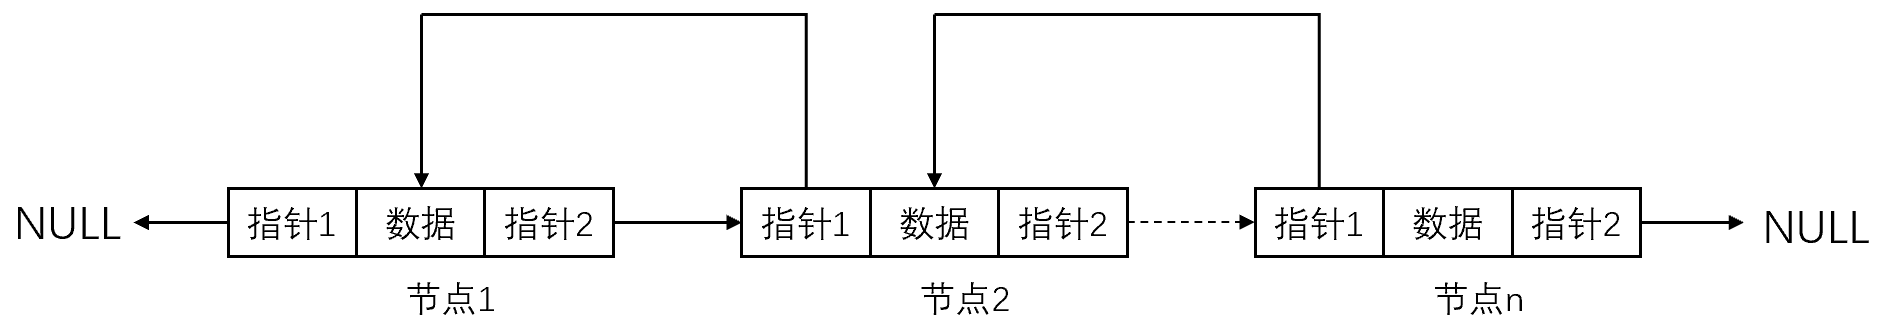
\includegraphics[width=0.78\textwidth]{assets/pics_and_ppts/ch2/双链表示意图.png}
    \caption{双链表示意图}
    \label{fig:双链表示意图}
    
\end{figure}

这样，我们就能以O(1)时间立即找到某个给定节点的前驱节点。同时新增的节点也带来的编码上的不同，比如，在插入、删除节点时，要多维护一个指针（一个很有趣的事实是，你以为
这是让编码更加复杂，但实际上是更加简单。相信在你填充了代码\ref{code:双链表的插入操作}和代码\ref{code:双链表的删除操作}之后会深有体会）。
\begin{thinkbox}
    双链表可不可以带头节点？若不能，为什么？若可以，带头结点会有和单链表类似的好处吗？\\
    双链表的以下操作时间复杂度是多少？\\
    1. 插入操作；2. 删除操作； 3. 按位序访问； 4.按值访问； 5. 求表长。
\end{thinkbox}
正如笔者一再指出，对《数据结构》的研究和学习应该是“重在培养能力”。大家通过前面的研究，熟悉了单链表的思想之后，
应该能较轻松地写出双链表相关操作的代码。因此，笔者在这里进行第一次“留白”，请大家自行实现双链表操作的代码，并分析时间空间复杂度。

\minisection{1.双链表的插入操作}
时间复杂度：$\underline{\hspace{1cm}}$，空间复杂度：$\underline{\hspace{1cm}}$。
\begin{cppcodeNum}[label={code:双链表的插入操作}, codetitle={双链表的插入操作}, showlinenumber=false]
// 在双链表L中，第index个位置插入一个值为e的元素. DL: Double Linked.
    void DLListInsert(ListNode* L, int index, ElemType e) {
        












    }
\end{cppcodeNum}
\minisection{2.双链表的删除操作}
时间复杂度：$\underline{\hspace{1cm}}$，空间复杂度：$\underline{\hspace{1cm}}$。
\begin{cppcodeNum}[label={code:双链表的删除操作}, codetitle={双链表的删除操作}, showlinenumber=false]
// 在双链表L中，删除第index位置的元素。
    void DLListDelete(ListNode* L, int index) {
        
    











    }
\end{cppcodeNum}

这里笔者仅提示一点：我们在\ref{subsec:插入和删除}曾经指出，在已经拿到待删节点指针的情况下，单链表的删除操作的时间复杂度仍然为O(n)。但是双链表却不同，在已经
拿到待删节点指针的情况下，可以达到O(1)的时间复杂度。

\subsection{循环链表}
如果让单链表的表尾节点的后继指针指向表首节点，而不是NULL，这就成为了一个\term{循环单链表}，如图\ref{fig:循环链表示意图} a）；类似地，
将双链表的表首节点的前驱指针指向表尾节点，同时将表尾节点的后继指针指向表首节点，而不是NULL，就成为了\term{循环双链表}，如图\ref{fig:循环链表示意图} b）。
\begin{figure}[htbp]
    \centering
    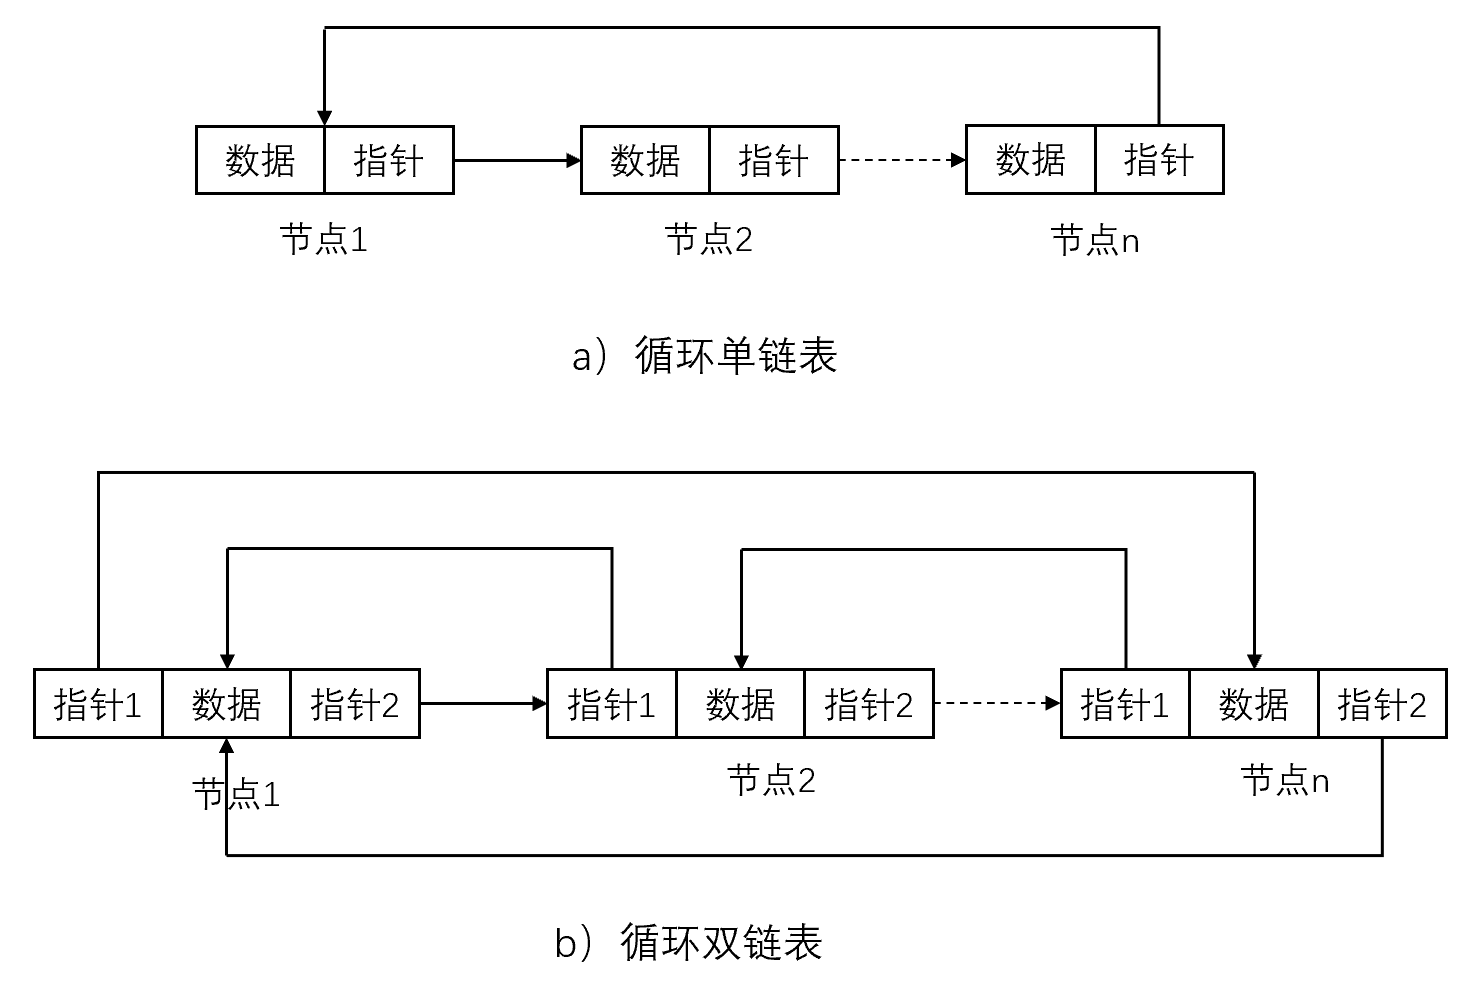
\includegraphics[width=0.78\textwidth]{assets/pics_and_ppts/ch2/循环链表示意图.png}
    \caption{循环链表示意图}
    \label{fig:循环链表示意图}
\end{figure}
可以看出，循环链表由于其循环的特性，给出其任一位置的指针，都可以顺着该指针遍历链表。在这里，我们指出两点循环链表带来的好处。

1. 与普通双链表相比，循环双链表可以在O(1)时间完成尾插。

2. 事实上对于循环单链表来说，保存尾指针（而不是头指针）通常是一种更好的做法，因为有了尾指针p，即可以通过p->next立即找到头指针。并且保存尾指针的循环单链表在
表头和表尾插入元素都可以在O(1)时间实现。

\subsection{静态链表}
实际需求中，有些场景需要频繁地创建、销毁对象，如某空战游戏，战机频繁地打出子弹，子弹碰撞到某物体后或飞出屏幕外之后消失。这种场景下，如果我们频繁地调用
malloc/free就会产生较严重的内存分配开销以及内存碎片（相信如果你学习过《操作系统》就会对此有深刻理解）。这种场景：1. 普通链表非常适合频繁插入删除，
但链表的动态节点分配机制，在高频创建/销毁场景下带来了额外开销； 2. 顺序表又不适合频繁地插入删除。

所以这个时候，\term{静态链表}就可以派上用场。如图\ref{fig:静态链表示意图}所示，静态链表将链表中的所有节点存放在一个数组中。使用数组中的位置编号（下标）
来模拟指针，从而实现节点之间的链接关系。对于单链表，若某节点的后继指针指向NULL说明该节点是表尾节点。而静态链表，通常用一个不存在的下标（如-1）表示没有下一个节点了。
\begin{figure}[htbp]
    \centering
    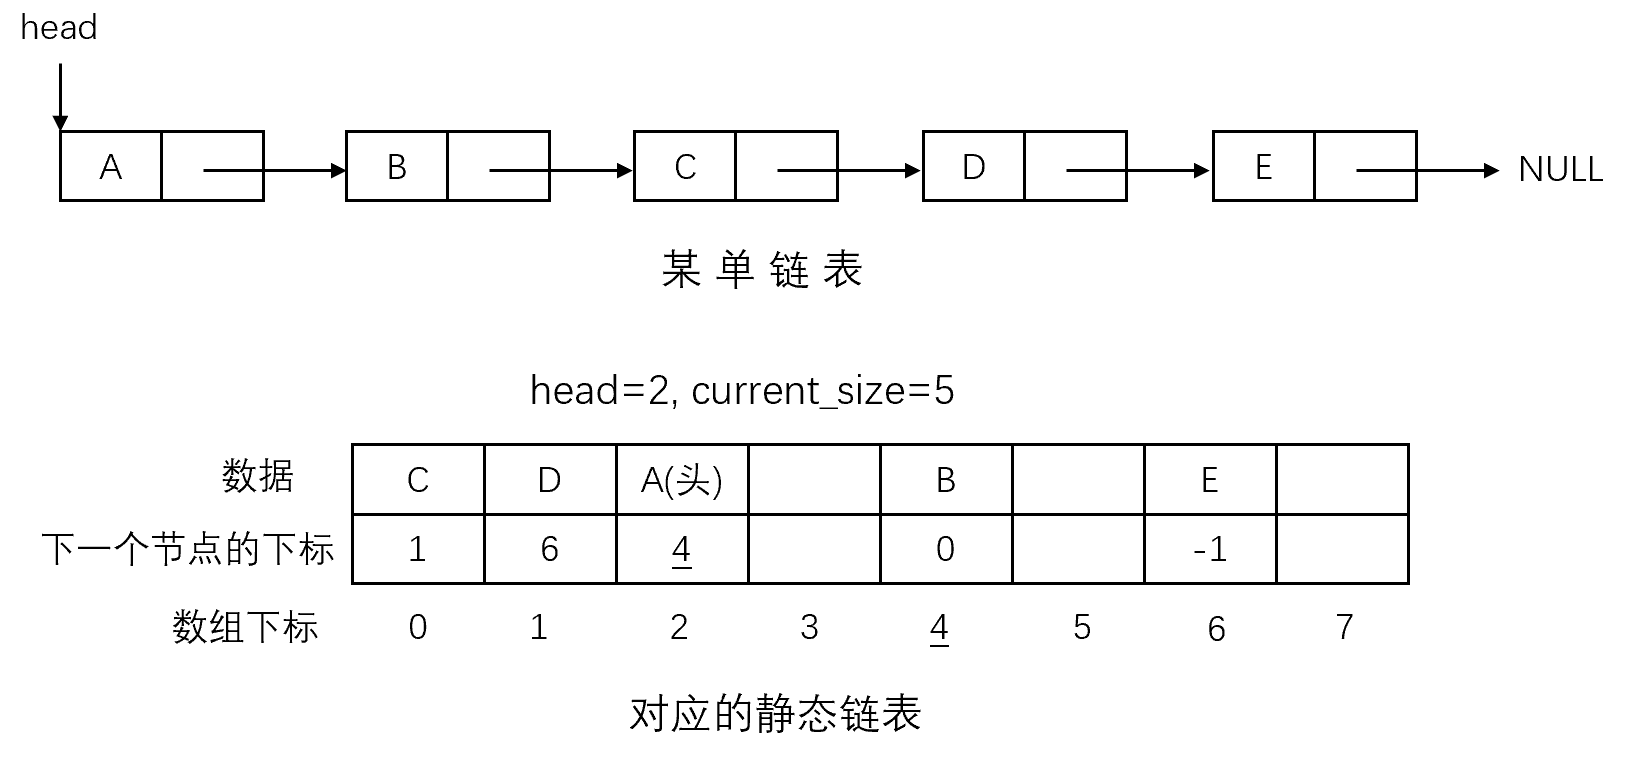
\includegraphics[width=0.78\textwidth]{assets/pics_and_ppts/ch2/静态链表示意图.png}
    \caption{静态链表示意图}
    \label{fig:静态链表示意图}
\end{figure}

静态链表的一个节点的存储结构如以下代码所示：
{
\setminted[cpp]{texcomments=true}
\begin{cppcodeNum}[label={code:静态链表的节点定义}, title={静态链表的节点定义}, minted options app={texcomments}]
    typedef struct {  
        ElemType data;  // 对应图 \ref{fig:静态链表示意图} 中的“数据”
        int next_node;  // 对应图 \ref{fig:静态链表示意图} 中的“下一个节点的下标”
    }SLinkListNode;
\end{cppcodeNum}
}

普通链表可以用其第一个节点的指针表示链表对象，对于静态链表，如何知道数组中哪个节点是第一个节点呢？一种做法是进行类似如下的封装：
\begin{cppcode}
    struct SLinkList {
        SLinkListNode data[MaxSize];    // 存放链表中节点的数组
        int current_size;   // 当前链表中的节点数量
        int head;   // 第一个节点所在的下标 
    }
\end{cppcode}
这样，我们便可以通过如下代码初始化一个静态链表：
\begin{cppcode}
    SLinkList L;
    L.current_size = 0;
    L.head = -1;    // 目前是空表 
\end{cppcode}
静态链表的其他操作，感兴趣的同学可以自行尝试实现。

\section{本章小结}
“\term{数据结构}是相互之间存在一种或多种特定“关系”的数据元素的集合，以及定义在这些数据元素上的“操作”的集合。“数据结构”的物理存储、操作通常通过计算机语言来实现。”
相信通过本章的探讨，大家已经能进一步理解这句话的含义。“线性表”作为一种逻辑结构，要求数据元素之间有“位置关系”，每个节点（除表尾节点）有且仅有一个直接后继，每个
节点（除表首节点）有且仅有一个直接前驱。而顺序表和链表是线性表的两种不同实现方式，分别将线性表的元素以不同的物理结构存储，并通过不同手段建立元素间的逻辑关系。

\term{笔者再次强调}，研究数据结构的核心，并不是掌握某一种数据结构的代码，而是理解如何组织数据、如何分析问题、如何设计解决方案。以链表为例，我们学习的并不仅仅是：

-  链表的定义是什么；

-  链表有哪些操作；

-  创建一个结点的代码是什么； 

-  插入和删除操作的代码是什么； \\
更重要的是理解：

-  为什么需要链表的存在，它能解决什么问题？

-  为什么链表不需要连续的存储空间； 

-  为什么它能够高效地完成插入和删除；   

-  为什么它无法像数组一样快速随机访问； 

-  如何根据问题特点，在灵活性和效率之间进行选择。 \\
因此，学习数据结构时，不要只关注“这个结构怎么实现”（虽然这固然重要），而更应该思考：

-  为什么要这样设计？

-  它解决了什么问题？

-  它付出了什么代价？

-  如果换一种设计，会发生什么变化？\\
当你能够从这些角度理解一个数据结构时，你掌握的就不再只是链表、栈、队列或者树，而是一种分析问题和设计方案的能力。
这也是学习数据结构最重要的意义。
